\documentclass[11pt,fleqn]{article}

\usepackage{latexsym}
\usepackage{amssymb}
\usepackage{stmaryrd}
\usepackage{amsfonts}
\usepackage{amsmath}
\usepackage{url}

% Allow more line breaks in URLs
\usepackage{xurl}

% Enable links within the document
\usepackage{hyperref}
\usepackage{titlesec}

\usepackage[
  a4paper,
  top=3.8cm,
  bottom=2.5cm,
  inner=2.5cm,
  outer=2.5cm,
  headheight=15pt,
]{geometry}

\hypersetup{
  colorlinks=true,
  linkcolor=red,
  urlcolor=red,
  breaklinks=true,
}
\urlstyle{rm} % Make URL styled fonts match hyperref's hrefs

\usepackage{cleveref}

% Credit to Gabriel Devenyi for this bibliography cfg:
% github.com/gdevenyi/mcmaster.latex
\usepackage[
  style=numeric-comp,
  backend=biber,
  sorting=none,
  backref=true,
  maxnames=99,
  alldates=iso,
  seconds=true
]{biblatex} % bibliography
\addbibresource{references.bib}

% Soure code
\usepackage{listings}

\Crefname{lstlisting}{Listing}{Listings}

\lstdefinestyle{mystyle}{
  basicstyle=\ttfamily\footnotesize,
  tabsize=2,
  columns=fullflexible,
  breaklines=true,
  postbreak=\mbox{\textcolor{red}{$\hookrightarrow$}\space},
}
\lstset{style=mystyle}

\title{\vspace{-3.5cm}CAS 703 Term Project: Validated General-Purpose Calculators}
\author{Hassan Zaker \and Jason Balaci}

\date{
	McMaster University \\ \texttt{\{zakerzah, balacij\}@mcmaster.ca}\\%
	\today
}

\usepackage{multicol}
\usepackage{todonotes}

\begin{document}

\maketitle

\tableofcontents

\lstlistoflistings

\newpage{}

%------------------------------------------------------------------------------
% Introduction
%------------------------------------------------------------------------------
\section{Introduction}
\label{sec:introduction}

For our term project in CAS 703~\cite{Paige7032023}, we decided to build a
language for describing calculation schemes. The descriptions should be mostly
understandable to anyone who has worked with Excel~\cite{Excel} or has used any
kind of calculation software. We aim to validate the
coherence\footnote{``Coherence'' defined by an unambiguous set of constraints
and rules.} of the calculator descriptions. Additionally, through generative
techniques, we hope to decrease the barrier to entry (as much as we can) of
basic software development of calculator programs by defining a transformation
of the calculator descriptions to various programming
languages\footnote{Notably, Java programs.}.

\subsection{Objective}
\label{sec:introduction:subsec:objective}

We aim to:

\begin{enumerate}

  \item design a metamodel for describing calculator programs
        (\Cref{sec:modelling}),

  \item build a concrete syntax for the metamodel, and an Integrated Development
        Environment (IDE) for said concrete syntax
        (\Cref{sec:integrated-development-environment}),

  \item design a set of rules that define ``coherence'' rules of the metamodel
        and audit instances of the metamodel for coherence
        (\Cref{sec:model-validation}), and

  \item define a transformer that converts the calculator description into
        programs and corresponding documentation
        (\Cref{sec:model-management-operations}).

\end{enumerate}

\subsection{Tooling}
\label{sec:introduction:subsec:tooling}

We will use the tooling shown in 703, namely: Eclipse Epsilon~\cite{Epsilon} and
the languages it contains, and Xtext~\cite{Xtext}.

\newpage{}

%------------------------------------------------------------------------------
% Modelling
%------------------------------------------------------------------------------
\section{Modelling}
\label{sec:modelling}

To define our metamodel for our desired Domain-Specific Language (DSL), we first
need to iron out the \textit{requirements} of that language.

\subsection{Requirements}
\label{sec:modelling:subsec:requirements}

When we (the authors) think of ``calculators,'' we think of 3 main components:
(i) a set of input symbols, (ii) a set of output symbols, and (iii) a means of
deriving the output symbols from the input symbols. (i) and (ii) are really just
``symbols'' with designation of whether they are user-provided or calculated.
(iii) is a (commonly secret) algorithm that translates (i) to (ii) and which may
rely on intermediate symbols irrelevant to (i) and (ii). Thus, we think of a
calculator as being a structure of (a) symbols of different kinds (inputs,
intermediates, and outputs) and (b) an algorithm that calculates some symbols
from an initial subset of provided symbols.

Depending on your preferred school of thought, algorithms can be thought of
differently. We choose to think of them as being similar to imperative-style
programming languages, where there is a memory of symbols to values, and a
sequence of steps/statements that are executed sequentially against the memory.

The most important kind of ``step'' our algorithm must have is ``symbol
assignment,'' where some symbol is assigned the value of some expression. The
expression may contain other symbols, but it should be restricted to only using
symbols that have been assigned values (either as input to the calculator or by
an earlier step). Logging is another important kind of step that algorithms
might need, they're typically used for providing user-feedback for debugging,
general information, warnings, errors, etc. Logging, similar to assignment
steps, are provided an expression, for which are evaluated, but the difference
is that the logging step displays the value to the user-feedback mechanism of
the calculator rather than assigning the value to a symbol. For now, we choose
to think of calculators as only having these 2 kinds of steps.

The steps rely on a single mathematical expression language that describes how
values can be altered in a predictable way. We choose to restrict our expression
language to the common first-order definite-valued mathematical language that
most undergraduates in a first-year university mathematics class are familiar
with.

Similar to how we expect our expression language to provide predictable results,
we also expect our calculators to be predictable and reliably produce accurate
results. To gain confidence in accuracy and predictability, we can test our
calculators against well-known outputs for well-known inputs. In other words, we
can create test cases to gain confidence that our calculator is reliable (which
we want to reasonably assure ourselves).

Thus, together, we define our calculator as having 3 main aspects: (a) a set of
symbols, (b) an algorithm that somehow calculates the output symbols from the
inputs, and (c) a set of test cases to gain confidence that (b) is reliable. To
model our calculator DSL, we chose to use Emfatic (EMF) because we found it to
be faster to work with. In particular, we found it to be more readable and
easier to modify compared to Ecore.

\subsection{Emfatic}
\label{sec:modelling:subsec:emfatic}

\begin{lstlisting}[caption={Calculator EMF},label={lst:calculator}]
class Calculator extends Described {
  attr String[1] name = "";
	val SymbolDeclaration[*] symbolDeclarations;
	val CalculationStep[*] steps;
	val TestCase[*] testCases;
}
\end{lstlisting}

When translating the calculators to Emfatic (\Cref{lst:calculator}), we also
added the name and a description of the calculators using string
attributes\footnote{Note that since we commonly use comments and descriptions,
we added a ``Described'' base class to quickly attach description attributes
(\Cref{lst:described}).}. The calculator class contains 3 other ``containment
references'' (\lstinline{val}s): symbol declarations, calculation steps
(denoting the algorithm), and a set of test cases.

Symbol declarations (\lstinline{SymbolDeclaration},
\Cref{lst:symbol-declarations}) define a symbol (\lstinline{Symbol}) with a
textual description and the \textit{kind} of symbol it is \textemdash{} input
(user-provided at the start of the calculator), intermediate (derived from the
inputs but not important), or output symbols (symbols that users are interested
in calculating). Since the difference between the symbol kinds is quite surface
level (or so we claim), we chose to use an \lstinline{enum} attribute in our
symbol declaration type. If there were any behavioural differences, we would
have used a subclass. The symbol content itself is contained in another class
(\lstinline{Symbol}) with a one-to-one relationship with symbol declarations.
\lstinline{Symbol}s contain a name attribute (assumed to be a Java-friendly
identifier) and a declared \textit{type} of the symbol. The types are
containment references of \lstinline{Type}s (\Cref{lst:type-universe}).  

We chose to build a basic unambiguous, static,
judgment-based~\cite{nlab:judgment} type system. We restricted our type universe
in our calculator to ``simple'' first-order types with no parameters. Thus, we
have booleans, strings, integers, and real numbers. However, we do intend to
implement vectors as well. We used an abstract \lstinline{Type} class to create
a generic class of types (with basic feature requirements), and then a subclass
(\lstinline{PrimitiveType}) to designate primitive types using an enumeration of
primitive types (\lstinline{Primitive}). By extending the basic \lstinline{Type}
class with other types, we can further extend our DSLs type system.

The next major component of our calculators are the calculation steps. As
already mentioned in \Cref{sec:modelling:subsec:requirements}, we restricted
ourselves to 2 kinds of steps: assignment steps, and print steps. Assignment
steps (\lstinline{AssignmentStep}) and print steps (\lstinline{PrintStep}) are
both subclasses of the abstract base class: \lstinline{CalculationStep}
(\Cref{lst:calculation-steps}). Print steps contain a description (we called it
a ``preface'') for the need to print a particular symbol (noted by reference).
\lstinline{AssignmentStep}s contain a reference to a symbol, an optional
description \lstinline{String} attribute, and a value reference to a defining
expression. The expression is expected to be well-typed, but we only impose this
restriction in \Cref{sec:model-validation}.

Expressions have a shared base class: \lstinline{Expression}
(\Cref{lst:expression-language}). There are various kinds of expressions we've
implemented, such as literals (\lstinline{TextLiteral},
\lstinline{BooleanLiteral}, \lstinline{IntegerLiteral},
\lstinline{RealLiteral}), symbol references (\lstinline{SymbolExpression}),
unary expressions (\lstinline{UnaryExpression}), binary expressions
(\lstinline{BinaryExpression}), and tertiary expressions
(\lstinline{TertiaryExpression}). The \lstinline{Expression} abstract base class
defines a basic functionality set that each subclass of expression must provide
\textemdash{} namely printing, type inference, symbols it depends on, and a Java
representation method.

The last component of our calculators are test cases. We expect that instances
of these calculators to obey a set of test cases. Our \lstinline{TestCase} class
is defined with a name and description String attributes, a list of assignment
steps (that are expected to reference no symbols in their expressions), and a
list of boolean-typed expressions\footnote{Both restrictions are only imposed in
\Cref{sec:model-validation}.}.

Finally, these 3 important classes define our calculators, and we may continue
to our next project: building a concrete syntax for our DSL.

\newpage{}

%------------------------------------------------------------------------------
% IDE
%------------------------------------------------------------------------------
\section{Integrated Development Environment}
\label{sec:integrated-development-environment}
We decided to use Xtext to build our IDE because the nature of our program usage
is not graphical, it is very mathematical, and so we felt text was best. At
first, we developed an IDE using Xtext that worked fine, but it was not
connected to our metamodel. Then we struggled to connect it to our metamodel,
and so we had to restart our Xtext project, basing it on our
``metamodel.genmodel'' file. The concrete syntax looks like \Cref{fig:ide1}, and
the full concrete syntax is in the appendix.

   \begin{figure}[h]
    \centering
    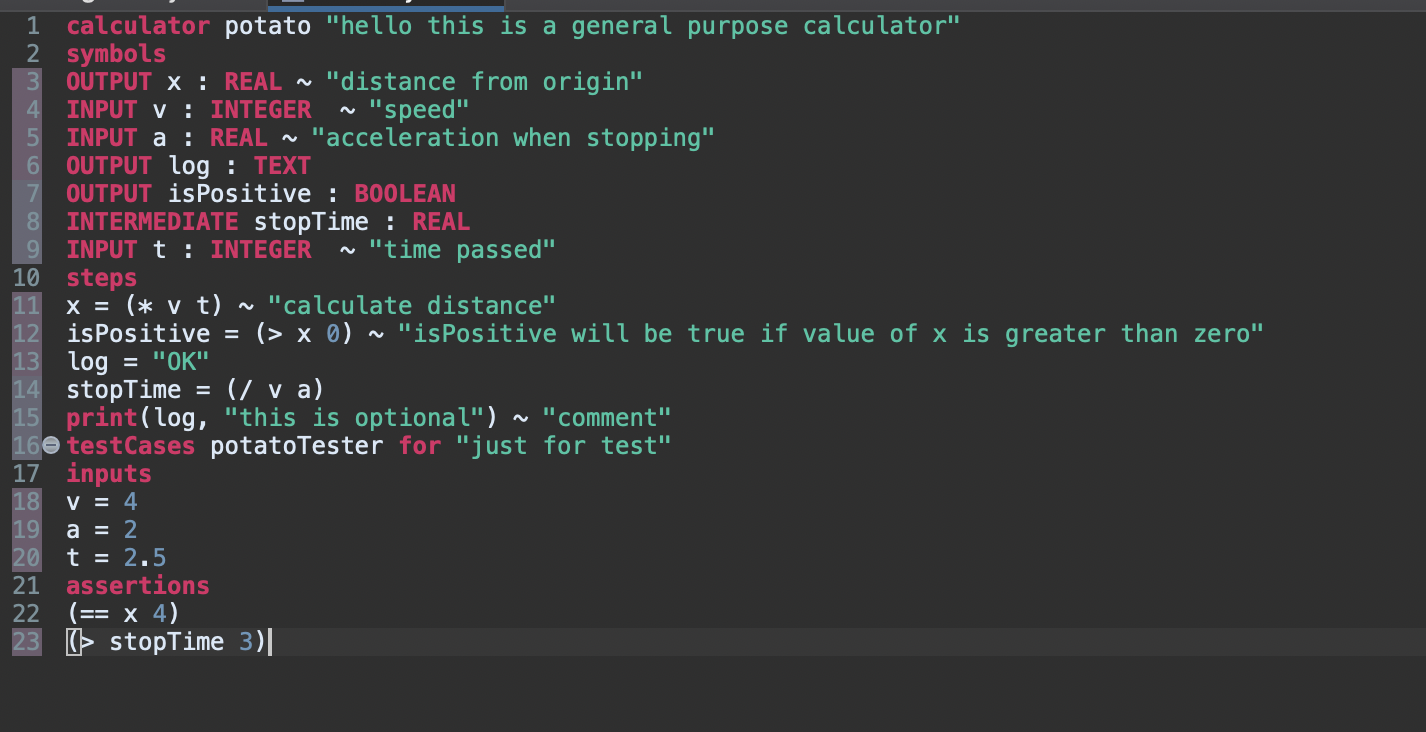
\includegraphics[width=1\textwidth]{ide1.png}
    \caption{A simple example of our calculator in our IDE}
    \label{fig:ide1}
\end{figure}

\noindent{}Design Decisions:
\begin{enumerate}

  \item Connecting Xtext to our metamodel forced us to do some modifications in
        our pre-existing syntax. One of this changes for the symbol kind. In the
        symbol declaration section, each symbol should be associated to one of
        three kinds (INPUT, INTERMEDIATE, OUTPUT). Our first choice was to have
        three subsections (one for each kind), and every symbol should be
        defined in the corresponding subsection\footnote{For example, a section
        for input variables, intermediate variables, and output variables.}.
        However, after connecting Xtext to our metamodel, we were not able to do
        that because we had to set a default value for
        \lstinline{SymbolDeclarationKind} attribute in
        \lstinline{SymbolDeclaration} class and Xtext does not allow us to
        assign information without consuming some sort of text (which we didn't
        want to have) even though our grammar was still context-free. Now, all
        symbols are defined in one ``symbols'' section with their kind manually
        specified for each of them. See lines 2-9 in \Cref{fig:ide1} for
        example, we originally wanted the kinds of symbols to be separated into
        blocks of symbols.
  
  \item One other modification we had to make for the same problem with enums
        was for expressions. In the first xtext project(the one that was not
        connected to metamodel) we implemented expressions very well. Precedence
        of every expression was considered. We tried to do the same thing here
        (xtext connected to metamodel) but it was not possible since we were not
        able to assign a default value to the operation attribute(which is an
        enum). Therefore, we decided to change the syntax for expressions to
        s-expressions.

\end{enumerate}
  
Beside the rules that are defined in the grammar, we defined three validation
rules in our IDE. Checking these rules was not possible without adding special
validation rules to Xtext. If users don't follow these rules, they will see a
corresponding error (see \Cref{fig:ide2} for example).

\begin{figure}[h]
  \centering
  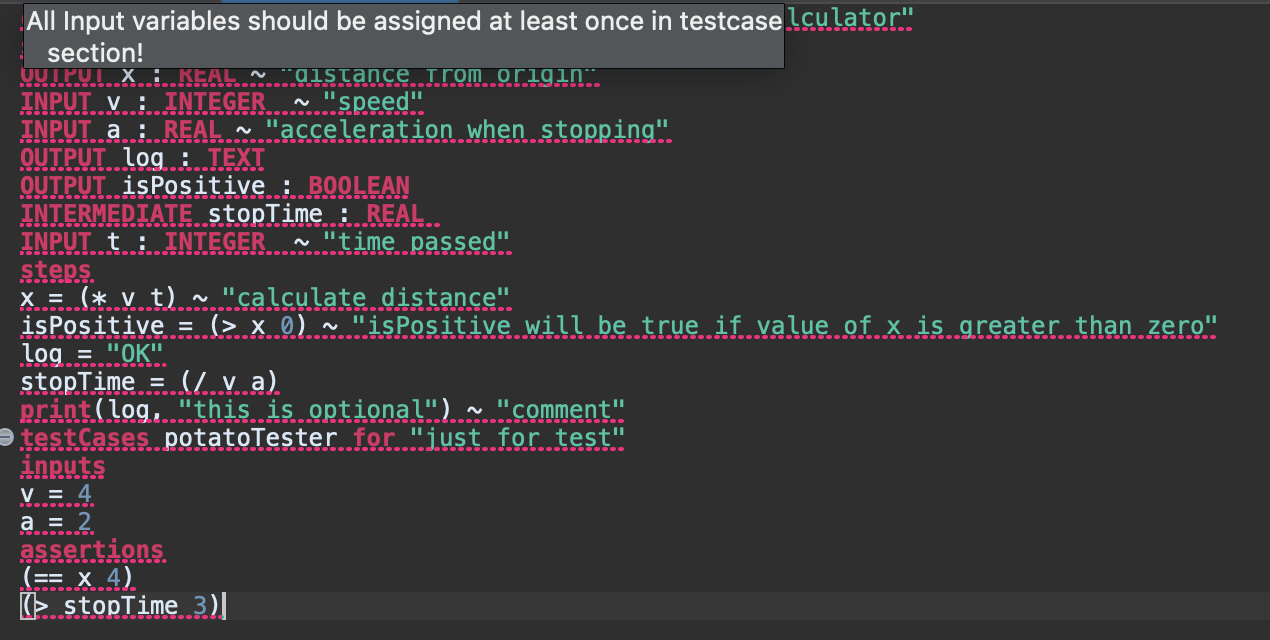
\includegraphics[width=1\textwidth]{ide2.png}
  \caption{Validation error in our IDE}
  \label{fig:ide2}
\end{figure}

\noindent{}Validation Rules incorporated in our IDE:
\begin{enumerate}

  \item Every symbol must have a unique name.

  \item Every symbol with output or intermediate kind must be assigned at least
        once in the steps section.

  \item Output and intermediate symbols should not be assigned in test case
        section.

  \item Every input symbol must be assigned a value in test case section.

  \item Using any symbol's name in steps or test case section that is not
        already defined is not allowed.

\end{enumerate}

Unfortunately, as we had left our IDE development to our last step in our DSL
development, not all of our validation rules appear in our IDE. However, we do
hope to integrate them soon in full.

\newpage{}

%------------------------------------------------------------------------------
% Model Validation
%------------------------------------------------------------------------------
\section{Model Validation}
\label{sec:model-validation}

Using the Epsilon Validation Language (EVL), we built a series of constraints to
impose restrictions we weren't able to adequately impose through the metamodel
(\Cref{lst:constraints-and-critiques}). In particular, we built a series of
constraints (hard requirements) and critiques (soft requirements/preferences)
for models of our metamodel.

\noindent{}Calculator Constraints:
\begin{enumerate}
  \item \textit{named}: each calculator must have a name for users to
        disambiguate between calculators and their other files,
  \item \textit{unique symbols}: each calculator must have a set of symbols that
        have unique names within that set so variable references can be
        unambiguous,
  \item \textit{at least 1 input}: each calculator should have at least 1 input
        symbol or else there is no interactivity with the calculators generated,
        so a normal calculator should be used instead,
  \item \textit{at least 1 output}: each calculator should have at least 1
        output symbol or else there would be no way to audit or use the
        calculator,
  \item \textit{all outputs assigned once}: all designated output symbols are
        meaningful in some way and should be guaranteed to have a value at the
        end of the calculation steps,
  \item \textit{all intermediate symbols assigned once}: if a declared
        intermediate symbol is never assigned, then it can be removed to
        de-clutter the calculator,
  \item \textit{all assignment steps well-typed}: each assignment should involve
        a symbol of the same type as an expression,
  \item \textit{all test case assignments are input symbols}: the
        pre-calculation state of the calculators should only have input
        variables assigned values,
  \item \textit{all test case assignments contain no variable references}: all
        assignment bodies in test cases should be evaluable to literal-valued
        expressions (e.g., contain no symbol references) because there is no
        defined variables before input set,
  \item \textit{all test cases assign all input variables}: each test case
        should mimic users fully, by providing all necessary inputs the
        calculator would need,
  \item \textit{all test case inputs unambiguous/``no duplicates''}: each
        defined test case should have no ambiguous symbol assignments or else
        the initial state of the test case simulations would be ambiguous,
  \item \textit{all test case assertions are boolean-typed}: the assertions
        should be propositional statements or else they should be part of the
        calculation steps of the main calculator,
  \item \textit{all steps depend on non-null symbols}: each step of the
        calculation should only rely on symbols with defined values or else
        invalid and undefined expressions and operations will occur, and
  \item \textit{all test cases satisfied}: the calculation steps should be
        simulated under each test case, and each test case should be satisfied.
\end{enumerate}

\noindent{}Calculator Critiques:
\begin{enumerate}
  \item \textit{description}: it would be nice to have a description of the
        intent of the calculator and general information about how it works,
  \item \textit{all inputs described}: it would be nice for each input symbol to
        have a user-friendly description to describe what the variable means,
  \item \textit{all outputs described}: same as above, and
  \item \textit{all test case assertions meaningful}: each test case assertion
        statement should reference symbols in that calculator or else the
        assertion would be evaluable without simulation.
\end{enumerate}

\noindent{}Symbol constraints:
\begin{enumerate}
  \item \textit{named}: each symbol should have a name or else using them would
        be impossible, and
  \item \textit{named with only appropriate characters}: a restriction imposed
        by desiring Java-compilation and non-unicode data entry \textemdash{}
        names/identifiers should be usable as Java identifiers.
\end{enumerate}

Finally, we have our last constraint: each expression should be well-typed, or
else invalid states are possible, and we don't want calculators to ever get
``stuck.''

Together, these make up our constraints. We build them using standard EVL
tooling (\Cref{lst:constraints-and-critiques}) and run them using a Gradle
script on our parsed model. If all constraints and critiques are satisfied for a
model, then we claim that the produced artifacts (see
\Cref{sec:model-management-operations}) and the model are relatively
high-quality. Furthermore, we claim that the produced code artifact should be
well-typed, and thus never run into invalid states, errors, or any issue at
runtime (excluding that related to business logic).

The simulation of the test cases is one of our larger validation schemes. We had
to emulate the Java code that would be run under the test cases provided.
Unfortunately, we were not able to add an ``evaluation'' method to the base
\lstinline{Expression} class because we needed the return type of the function
to be \lstinline{Any}. We wanted to use \lstinline{Any} because we wanted to use
the dynamic typing nature of EOL to avoid model duplication for literal values.
However, the EMF language does not support \lstinline{Any}, and thus we had to
``attach'' this functionality post-facto in our shared ``program.eol'' file used
by all of our other files. For simulating the calculation steps, we faced
similar issues with our base \lstinline{TestCase} type. We had to have an
implicitly known base property of test cases that they are simulatable. For
expressions, our evaluation methods were given an (implicitly) read-only
``scope'' Map for them to reference symbols. Similarly, for our simulation, we
also had to pass along the current variable state of the simulation memory.
However, the calculation steps are allowed to read from and modify the scope.
The full code for simulation works by populating an initial memory state with
the input variables, executing the calculation steps on the memory, and then
checking that all the provided assertion propositions hold true
(\Cref{lst:simulation-specific-code}, specifically the \lstinline{isSatisfied}
operation).

Another notable constraint is the dependency-checking of each calculation step
\textemdash{} that is, each step should only rely on symbols that are reasonably
guaranteed\footnote{``Division by 0,'' and other issues that would require a
dependent type system to mitigate are not considered.} to have been assigned a
value already. In order to validate, we had to iterate over the calculation
steps sequentially, processing what impact they would have on symbols and what
symbols they rely on to decide whether they are okay or not
(\Cref{lst:check-step-dependencies}). The initial set of valid usable symbols
are only the input symbols, and it is expected that by the end, each output
symbol is calculated. The remainder of the validation rules rely on asserting
propositions over all instances of data types, mostly with respect to a
particular calculator, using the standard primitive tooling available in EOL and
EVL. Finally, with the validated models, we may build our desired artifacts.

\newpage{}

%------------------------------------------------------------------------------
% Model Management Operations
%------------------------------------------------------------------------------
\section{Model Management Operations}
\label{sec:model-management-operations}

As mentioned in \Cref{sec:introduction:subsec:objective}, our final objective is
to realize the calculator models into vetted, usable programs for end users.
Ultimately, our goal is that the program should be simple enough that any
computer user may be able to use the generated programs. However, this
requirement requires a lot more work to assure user-friendliness across
audiences, portability across various operating systems, and may involve a
Graphical User Interface (GUI) or other modes of computer interaction. Thus, for
the time being, we restrict ourselves to building Command-Line Interface (CLI)
tools using a programming language that is already sufficiently portable (i.e.,
Java\footnote{Note that this requirement of Java required us to slightly adjust
our typing rules with generating Java code in mind! For example, until we build
our own standard library tooling, we weren't able to have integer exponentiation
since the \lstinline{java.lang.Math} package does not support integer powers
without casting.}). Additionally, to complement the CLI calculator tools we
generate, we also generate a ``read me'' file in Markdown (i.e., a
\lstinline{README.md} file). To generate both artifacts, we used 2 Epsilon
Generation Language (EGL) files alongside the EGL Co-Ordination Language (EGX)
to orchestrate their usage.

\subsection{Working with EGL}
\label{sec:model-management-operations:subsec:working-with-egl}

Working with EGL was quite enjoyable for us, we found little to no issues at all
using it. We chose to treat the target artifacts as ``text'' (hence using EGL)
rather than ``models'' (which would require encoding Markdown and Java models)
due to time constraints on the course and complexity associated with building a
full Java Abstract Syntax Tree (AST) in EMF. Thus, we performed model-to-text
model transformations. We built some extra tools in EOL to simplify our EGL
code, such as adding defaults for empty strings, expression conversion to
human-readable syntax, grabbing only the input/intermediate/output symbols, and
more. One difficulty faced is generating the human-readable expressions without
excessive parentheses. Ultimately, this was a constraint by time rather than by
knowledge or the Epsilon tools since we wanted to have a custom mathematic
notation for the end users of the programs. In other words, the human-readable
notation would be appear slightly different than the input calculator models.
However, it would have the same meaning and behaviour (and a bijection would
exist between them).

We fed in calculator instances to each of the EGL files and used that calculator
instance to grab all necessary information to generate each file (Java or
Markdown, respectively). The majority of the code involved (a) accessing
variables from the model, (b) pretty-printing the variables in-place as
necessary, and (c) adding default information and explanatory text where
applicable (such as when the model contains no intermediate symbols and we want
the user to know).

\subsection{Generating a Java Program}
\label{sec:model-management-operations:subsec:generating-a-java-program}

To generate our Java CLI programs, we built an EGL file
(\Cref{lst:java-generation-egl}) and hooked it up to our EGX
(\Cref{lst:egl-co-ordination}) to make sure we have a special folder to carry
our Java programs, one for each defined calculator. First, we manually built a
prototype calculator of what we wanted to build, and then we gutted out the
internal components that are accustomed to the model\footnote{In other words, we
abstracted over the data that was obtained from the model.} and regenerated them
using the input models. We used the Java standard library for scanning the
console for inputs from the user (via \lstinline{Scanner} usage on
\lstinline{System.in}), printing (via \lstinline{System.out.println}), and
certain non-standard calculations (via \lstinline{java.lang.Math}, such as
\lstinline{Math.pow} for powers). We setup the code to create a basic
introductory message and then immediately prompt users for the inputs (in the
order they are defined in the model). Afterwards, the code will define the
intermediate and output symbols, and run through the calculation steps
sequentially\footnote{In the future, we may be able to look to parallelization
and concurrency for large calculators.}. Finally, we print the value of each
defined output symbol at the end of the program, and it terminates. The program
is a single-file source program, so usage only requires a single
\lstinline{java Main.java} execution in your preferred shell. Hopefully in the
future we will be able to make this usage and interaction with the CLI programs
more user-friendly.

\subsection{Generating a README File}
\label{sec:model-management-operations:subsec:generating-a-readme-file}

Similar to our Java program generator, we also built an EGL file
(\Cref{lst:readme-generation-egl}) and hooked it up to our EGX
(\Cref{lst:egl-co-ordination}) to make sure we have a special folder to carry
our Java program along with the README files, specialized to each defined
calculator in the model. Again, we built a prototype README file and abstracted
over the details specialized to models. For example, we created variables for
the names, descriptions, input, intermediate, and output symbol tables,
calculation steps, and test case descriptions. Afterwards, we regenerated the
\lstinline{README.md} files using our EGL code. We made sure to include
documentation for the usage of the Java programs\footnote{With a target audience
of users comfortable with the command-line, such as Junior Programmers and Data
Analysts.}, a description of all the relevant variables to the program, a
description of the calculation steps the program takes, and the list of test
cases that were used to assert that the calculator models are reasonably
well-behaved.

Additionally, in both the Java program and the README files, we added some basic
accreditation information, noting that the software was built for educational
purposes under Dr.~Richard Paige's offering of CAS 703 at McMaster
University~\cite{Paige7032023}.

\newpage{}

%------------------------------------------------------------------------------
% Reflection and Concluding Thoughts
%------------------------------------------------------------------------------
\section{Reflection and Concluding Thoughts}
\label{sec:reflection-and-concluding-thoughts}

Ultimately, we greatly enjoyed working on this term project. Working with
Eclipse and Epsilon tooling was very enjoyable. The documentation for all
Epsilon tools was stellar, and the Epsilon Playground allowed us to play around
with the micro-models in isolated situations. 

We only found light, noticeable issues with \lstinline{enum} support across
tools, and with Xtext usage. Specifically, \lstinline{enum}s are not usable as
parameter types in operations in EOL, but are in EMF. The flexibility allowed by
the Epsilon tools was great, but the consistency here was problematic.
Similarly, in Xtext, enumeration values could not be defaulted for
constructions, which lead us to making an unfortunate decision to annotate our
symbol declarations with excessive ``input,'' ``intermediate,'' and ``output''
keywords (one per) for each declared symbol. Originally, we only wanted to have
a grouping of them where each block of symbols was contained in one of those
keyword blocks and assigned the related \lstinline{enum} value for the
declaration kind. Additionally, with Xtext, we found difficulty in debugging
issues related to our grammar and ended up needing to implement S-expressions
for our mathematical expression language so ease the issues and assure that we
could deliver for the deadline. We are confident that with more time, we would
be able to the appropriate mathematical expression language for the concrete
syntax, but for now, we are left with this.

On the side of Epsilon tooling, we found great enjoyment working with Gradle and
Ant to orchestrate the compiler. Originally, we developed an input model using
Flexmi and used that to drive development against calculators, and then we
worked towards adding Xtext to build a concrete syntax for our language. We
still preferred to keep the textual concrete syntax because a graphical language
we thought that defining expressions would be too time intensive for users.

In the future, we hope to (at least):

\begin{enumerate}
  \item further integrate our Gradle build script components with our
        Xtext-based editor,
  \item add extra support for vectors and more operations in our metamodel and
        concrete syntax, and
  \item generate more kinds of software artifacts (such as GUI-oriented
        programs, a single program that can connect multiple calculators, and
        interactive web-based Single Page Applications [SPAs]).
\end{enumerate}

Model-driven engineering, the underlying theory, and practical applications
thereof it, have been wonderful to learn about, and we hope to use these tools
and ideas in the future.

\newpage{}

%------------------------------------------------------------------------------
% Bibliography
%------------------------------------------------------------------------------
\printbibliography[heading=bibintoc]

\newpage{}

\section*{Appendix}
\addcontentsline{toc}{section}{Appendix}
\label{sec:appendix}

\begin{lstlisting}[caption={Abstract Class: Described},label={lst:described}]
abstract class Described {
  attr String[1] description = "";
}
\end{lstlisting}

\begin{lstlisting}[caption={Symbol Declarations},label={lst:symbol-declarations}]
class SymbolDeclaration extends Described {
  attr SymbolDeclarationKind[1] kind;
  val Symbol[1]#declaration symbol;
}

enum SymbolDeclarationKind {
  INPUT;
  INTERMEDIATE;
  OUTPUT;
}

class Symbol {
  id attr String[1] name = "";
  val Type[1] type;
  ref SymbolDeclaration[1]#symbol declaration;
}
\end{lstlisting}

\begin{lstlisting}[caption={Calculation Steps},label={lst:calculation-steps}]
abstract class CalculationStep extends Described {
	op String[1] toHRN();
	op Symbol[*] dependencies();
	op Symbol[*] calculates();
	op String[1] toJava();
}

class AssignmentStep extends CalculationStep {
	ref Symbol[1] symbol; // LHS
	val Expression[1] body; // RHS
}

class PrintStep extends CalculationStep {
	attr String[1] preface = "";
	ref Symbol[1] symbol;
}
\end{lstlisting}

\begin{lstlisting}[caption={Test Case},label={lst:test-case}]
class TestCase extends Described {
	attr String[1] name = "";
	val AssignmentStep[+] assignments;
	val Expression[+] assertions;
}
\end{lstlisting}

\begin{lstlisting}[caption={Type Universe},label={lst:type-universe}]
enum Primitive {
	TEXT;
	REAL;
	INTEGER;
	BOOLEAN;
}

abstract class Type {
  op String[1] serialize();
  op boolean[1] isNumeric();
	op String[1] toJavaType();
}

class PrimitiveType extends Type {
  attr Primitive[1] primitive;
}

class InvalidType extends Type {
  attr String[1] cause;
}
\end{lstlisting}

\begin{lstlisting}[caption={Expression Language},label={lst:expression-language}]
  abstract class Expression {
	op Type[1] type();
	op String[1] toHRN();
	op Symbol[*] symbolReferences();
	op String[1] toJava();
}

class TextLiteral extends Expression {
	attr String[1] value;
}

class RealLiteral extends Expression {
	attr double[1] value;
}

class IntegerLiteral extends Expression {
	attr int[1] value;
}

class BooleanLiteral extends Expression {
	attr boolean[1] value;
}

class SymbolExpression extends Expression {
    ref Symbol[1] symbol;
}

enum UnaryOp {
	LOGICAL_NOT;
	NEGATION;
}

class UnaryExpression extends Expression {
	attr UnaryOp[1] operator;
	val Expression[1] body;
}

enum BinaryOp {
	// numbers (of same type)
	ADDITION; // also allowed for text and vectors
	MULTIPLICATION;
	DIVISION;
	SUBTRACTION;
	POWER;
	MODULO;

	// inequalities
	GREATER_THAN;
	GREATER_THAN_EQUAL_TO;
	LESS_THAN;
	LESS_THAN_EQUAL_TO;
	
	// booleans
	LOGICAL_AND;
	LOGICAL_OR;
	LOGICAL_IMPLIES;
	
	// any
	EQUIVALENT;
	NOT_EQUIVALENT;
}

class BinaryExpression extends Expression {
  attr BinaryOp[1] operator;
  val Expression[2] exprs;
}

enum TertiaryOp {
  IF_THEN_ELSE;
}

class TertiaryExpression extends Expression {
  attr TertiaryOp[1] operator;
  val Expression[3] exprs;
}
\end{lstlisting}

\begin{lstlisting}[caption={Constraints and Critiques},label={lst:constraints-and-critiques}]
operation String withCalculator(c : Calculator): String {
    return c.name + ": " + self;
}

operation allUnique(c : Collection): Boolean {
    var asSet = c.asSet();
    return c.size() == asSet.size();
}

operation Collection hasDuplicates(): Boolean {
    return self.asSet().size() == self.size();
}

context Calculator {
    constraint NameLength {
        check: self.name.length() > 0
        message: "Calculator must have a name."
    }

    critique Description {
        check: self.description.length() > 0
        message: "It would be nice if you defined a human-readable description of your calculator.".withCalculator(self)
    }

    constraint UniqueSymbols {
        check: allUnique(self.symbols().name)
        message: "All symbols should have unique names.".withCalculator(self)
    }

    constraint AtLeast1Input {
        check: self.inputs().size() > 0
        message: "Each calculator should have at least 1 input.".withCalculator(self)
    }

    constraint AtLeast1Output {
        check: self.outputs().size() > 0
        message: "Each calculator should have at least 1 output.".withCalculator(self)
    }

    critique AllInputsDescribed {
        check: self.inputs().declaration.description.forAll(s|s.length() > 0)
        message: "Each input symbol should have a description for usability.".withCalculator(self)
    }

    critique AllOutputsDescribed {
        check: self.outputs().declaration.description.forAll(s|s.length() > 0)
        message: "Each output symbol should have a description for usability.".withCalculator(self)
    }

    constraint AllOutputsAssignedOnce {
        check: self.outputs().forAll(o|self.hasAssignmentStep(o))
        message: "Each output symbol should be assigned at least once in your calculation steps.".withCalculator(self)
    }

    constraint AllIntermediatesAssignedOnce {
        check: self.intermediates().forAll(o|self.hasAssignmentStep(o))
        message: "Each intermediate symbol should be assigned at least once in your calculation steps.".withCalculator(self)
    }

    constraint AllAssignmentsWellTyped {
        check: self.assignmentSteps().forAll(astep|astep.symbol.type.equiv(astep.body.type()))
        message: "Each assignment step must be well-typed.".withCalculator(self)
    }

    constraint AllTestCaseInputSymbolsAreInputs {
        check: self.testCases.forAll(testCase|testCase.assignments.forAll(asgn|asgn.symbol.declaration.kind==SymbolDeclarationKind#INPUT))
        message: "Test case inputs should only assign values to input variables".withCalculator(self)
    }

    constraint AllTestCaseInputExpressionsLiteral {
        check: self.testCases.forAll(testCase|testCase.assignments.forAll(asgn|asgn.body.symbolReferences().isEmpty()))
        message: "Test case inputs should not reference any symbol in their assignments.".withCalculator(self)
    }

    constraint AllTestCaseAssignAllInputs {
        // note: using '>=' here because (a) we already ensure that each symbol assigned is an input
        //       and that there are no duplicate assignments.
        check: self.testCases.forAll(testCase|testCase.assignments.symbol.size() >= self.inputs().size())
        message: "Test case inputs should assign a value to each input.".withCalculator(self)
    }

    constraint AllTestCaseInputsUnambiguous {
        check: self.testCases.forAll(testCase|testCase.assignments.symbol.hasDuplicates())
        message: "Test case inputs may not have ambiguous assignments for input symbols.".withCalculator(self)
    }

    constraint AllTestCaseAssertionsAreBooleanTyped {
        check: self.testCases.forAll(testCase|testCase.assertions.forAll(e|isBoolTy(e.type())))
        message: "Test case assertions must all be propositions (boolean-typed expressions)".withCalculator(self)
    }

    critique AllTestCaseAssertionsMeaningful {
        check: self.testCases.forAll(testCase|testCase.assertions.forAll(e|not e.symbolReferences().isEmpty()))
        message: "Each test case assertion should have at least 1 symbol reference, or else the check if superfluous".withCalculator(self)
    }

    constraint AllStepsDepsHaveValues {
        check: self.checkStepDependencies()
        message: "Each step's symbol dependencies must be satisfied before that step.".withCalculator(self)
    }

    constraint AllTestCasesSatisfied {
        guard: self.satisfiesAll("AllStepsDepsHaveValues", "AllTestCaseAssertionsAreBooleanTyped", "WellTyped", "AllIntermediatesAssignedOnce", "AllOutputsAssignedOnce")
        check: self.testCases.forAll(testCase|testCase.isSatisfied(self.steps))
        message: "Not all test cases are satisfied! Check algorithm!".withCalculator(self)
    }
}

context Expression {
    constraint WellTyped {
        check: self.isWellTyped()
        message: "Expression is ill-typed: " + self.type().serialize()
    }
}

context Symbol {
    constraint SymbolsNamed {
        check: Symbol.forAll(s|s.name.length() > 0)
        message: "All symbols must have a non-empty name"
    }

    constraint SymbolsNamedAppropriately {
        check: Symbol.forAll(s|s.name.matches("^[a-zA-Z]([a-zA-Z0-9_]+)?\$"))
        message: "All symbols must start with a letter and be followed by a sequence of letters, numbers or underscores."
    }
}
\end{lstlisting}

\begin{lstlisting}[caption={Simulation-specific Code},label={lst:simulation-specific-code}]
operation TextLiteral evaluate(scope : Map): Any {
    return self.value;
}

operation RealLiteral evaluate(scope : Map): Any {
    return self.value;
}

operation IntegerLiteral evaluate(scope : Map): Any {
    return self.value;
}

operation BooleanLiteral evaluate(scope : Map): Any {
    return self.value;
}

operation SymbolExpression evaluate(scope : Map): Any {
    return scope.get(self.symbol.name);
}

operation UnaryExpression evaluate(scope : Map): Any {
    var value = self.body.evaluate(scope);

    switch (self.operator) {
        case UnaryOp#LOGICAL_NOT:
            value = not value;
        case UnaryOp#NEGATION:
            value = - value;
    }

    return value;
}

operation BinaryExpression evaluate(scope : Map): Any {
    var left = self.exprs[0].evaluate(scope);
    var right = self.exprs[1].evaluate(scope);
    var value = null;

    switch (self.operator) {
	    case BinaryOp#ADDITION:
            value = left + right;
	    case BinaryOp#MULTIPLICATION:
            value = left * right;
	    case BinaryOp#DIVISION:
            value = left / right;
	    case BinaryOp#SUBTRACTION:
            value = left - right;
	    case BinaryOp#POWER:
            value = left.pow(right);
        case BinaryOp#MODULO:
            value = left.mod(right);
        case BinaryOp#GREATER_THAN:
            value = left > right;
        case BinaryOp#GREATER_THAN_EQUAL_TO:
            value = left >= right;
        case BinaryOp#LESS_THAN:
            value = left < right;
        case BinaryOp#LESS_THAN_EQUAL_TO:
            value = left <= right;
	    case BinaryOp#LOGICAL_AND:
            value = left and right;
	    case BinaryOp#LOGICAL_OR:
            value = left or right;
	    case BinaryOp#LOGICAL_IMPLIES:
            value = (not left) or right;
	    case BinaryOp#EQUIVALENT:
            value = left == right;
        case BinaryOp#NOT_EQUIVALENT:
            value = left != right;
    }

    return value;
}

operation TertiaryExpression evaluate(scope : Map): Any {
    var fst = self.exprs[0].evaluate(scope);
    var value = null;

    switch (self.operator) {
        case TertiaryOp#IF_THEN_ELSE:
            if (fst) {
                value = self.exprs[1].evaluate(scope);
            } else {
                value = self.exprs[2].evaluate(scope);
            }
    }

    return value;
}

operation AssignmentStep simulate(scope : Map): Map {
    scope.put(self.symbol.name, self.body.evaluate(scope));
    return scope;
}

operation PrintStep simulate(scope : Map): Map {
    var stub = self.symbol.name + " = " + scope.get(self.symbol.name).asString();
    if (self.preface?.length() > 0) {
        stub = stub + " ~ " + self.preface;
    }
    stub.println();
    return scope;
}

operation TestCase isSatisfied(progSteps : Collection): Boolean {
    // Create scope map
    var emptyScope = Map{};
    var scope = Map{};
    for (asgn in self.assignments) {
        scope.put(asgn.symbol.name, asgn.body.evaluate(emptyScope)); // note: each input should have an empty scope!
    }
    ("Testing assertion: " + self.name + ", with input set: " + scope.asString()).println();   
    
    // Simulate algorithm steps
    for (step in progSteps) {
        ("Simulating step: " + step.toHRN()).println();
        scope = step.simulate(scope);
    }

    // Evaluate assertions on the scope and ensure that they are all satisfied
    var allAssertionsSatisfied = true;
    for (assertable in self.assertions) {
        ("Checking assertion: " + assertable.toHRN() + "... ").print();
        if (assertable.evaluate(scope)) {
            "Ok!".println();
        } else {
            "Failed!".println();
            allAssertionsSatisfied = false;
            break;
        }
    }

    if (allAssertionsSatisfied) {
        ("Test case " + self.name + " SUCCEEDED!").println();
    } else {
        ("Test case " + self.name + " FAILED!").println();
    }

    return allAssertionsSatisfied;
}
\end{lstlisting}

\begin{lstlisting}[caption={Checking Calculation Step Dependencies},label={lst:check-step-dependencies}]
operation Calculator checkStepDependencies(): Boolean {
    var ok = true;
    var assigned = self.inputs().clone();

    for (step in self.steps) {
        if (not assigned.includesAll(step.dependencies())) {
            ok = false;
            break;
        }
        assigned.addAll(step.calculates());
    }

    return ok;
}
\end{lstlisting}

\begin{lstlisting}[caption={EGL Co-Ordination},label={lst:egl-co-ordination}]
pre {
    var artifactsDir = "../build/";
}

rule READMEs transform c : Calculator {
    template: "templates/readme.egl"
    target: artifactsDir + c.name + "/README.md"
}

rule JavaPrograms transform c : Calculator {
    template: "templates/java.egl"
    target: artifactsDir + c.name + "/Main.java"
}
\end{lstlisting}

\begin{lstlisting}[caption={Java Generation EGL},label={lst:java-generation-egl}]
[%import "../program.eol";%]
package Calculator;

// for reading inputs from standard input
import java.util.Scanner;

// for mathematical operations
import java.lang.Math;

/* This code is generated by Hassan Zaker and Jason Balaci as part of the course
 * requirements of CAS 703 (a graduate-level course at McMaster University, 
 * hosted by Dr. Richard Paige). 
 */
public class Calculator {

  public static void main(String[] args) {
    Scanner scanner = new Scanner(System.in);

    // introduction
    System.out.println("Welcome to the [%=c.name%] Calculator Program!");
    System.out.println("[%=c.description%]");
    System.out.println("Please see the related README.md file for more information.");

    // input symbols
[%for (input in c.inputs()) {%]
    System.out.println("Please input [%=input.name%] : [%=input.type.toJavaType()%]");
    [%if (input.declaration.description.length() > 0) {%]
    System.out.println(" ~ [%=input.name%] = [%=input.declaration.description%]");
    [%=input.type.toJavaType()%] [%=input.name%] = [%=input.type.javaReadCode()%];
    [%}%]
[%}%]
    scanner.close();

    // intermediate symbols
[%for (intmdt in c.intermediates()) {%]
    [%=intmdt.type.toJavaType()%] [%=intmdt.name%];
[%}%]

    // output symbols
[%for (o in c.outputs()) {%]
    [%=o.type.toJavaType()%] [%=o.name%];
[%}%]

    System.out.println("Calculating...");

[%for (step in c.steps) {%]
    [%=step.toJava()%];
[%}%]
    
    System.out.println("...ok!");

    System.out.println("Outputs:");
[%for (output in c.outputs()) {%]
    [%=output.type.javaPrintCode(output.name)%];
[%}%]
  }
}
[%
operation PrimitiveType javaReadCode(): String {
  var f;
	switch (self.primitive) {
		case Primitive#TEXT:
			f = "String";
		case Primitive#REAL:
			f = "Double";
		case Primitive#INTEGER:
			f = "Int";
		case Primitive#BOOLEAN:
			f = "Boolean";
	}
  return "scanner.next" + f + "()";
}

operation PrimitiveType javaPrintCode(s : String): String {
  return 'System.out.println("' + s + ' = " + ' + s + ')';
}
%]
\end{lstlisting}

\begin{lstlisting}[caption={README Generation EGL},label={lst:readme-generation-egl}]
[%import "../program.eol";%]
# [%=c.name%]
[%if (c.description.length() > 0) {%]
*[%=c.description%]*
[%}%]

## Software Guide

### Software Prerequisites

You should make sure to have a working installation of a Java compiler on your
system. This guide will assume you are using one of the standard Java tooling,
such as OpenJDK.

### Running the Calculator

The calculator is the standalone 'Main.java' file that is provided. To run it,
you should only need to run 'java Main.java' in your shell. If you prefer to
compile it into a Jar or a class file first, you should follow the instructions
provided by your installed Java development toolkit.

## Symbols

The [Inputs](#inputs) and [Outputs](#outputs) tables show variables relevant to
user interaction and usage of the [%=c.name%] calculator. The [Intermediates](#intermediates)
table shows variables strictly relevant to the underlying algorithm used for
deriving the outputs from the inputs.

### Inputs
[%var inputs = c.inputs();%]

[%if (inputs.size() == 0)  else {%]
| Symbol | Description | Type |
|:------:|:------------|:----:|
[%    for (s in inputs) {%]
| [%=s.name%] | [%=s.declaration.description.withDefault("—")%] | [%=s.type.serialize()%] |
[%    }%]
[%}%]

### Intermediates
[%var intermediates = c.intermediates();%]

[%if (intermediates.size() == 0)  else {%]
| Symbol | Description | Type |
|:------:|:------------|:----:|
[%    for (s in intermediates) {%]
| [%=s.name%] | [%=s.declaration.description.withDefault("—")%] | [%=s.type.serialize()%] |
[%    }%]
[%}%]

### Outputs
[%var outputs = c.outputs();%]

[%if (outputs.size() == 0)  else {%]
| Symbol | Description | Type |
|:------:|:------------|:----:|
[%    for (s in outputs) {%]
| [%=s.name%] | [%=s.declaration.description.withDefault("—")%] | [%=s.type.serialize()%] |
[%    }%]
[%}%]

## Calculation Steps
[%var steps = c.steps;%]

[%if (steps.size() == 0)  else {
    var sn = 0;
    for (step in steps) {
        sn += 1;%]
[%=sn%]. [%=step.toHRN()%]
    [%}
}%]

## Test Cases
[%var testCases = c.testCases;%]

[%if (testCases.size() == 0)  else {%]
The algorithm was tested in a simulation against the below test cases.
[%  var curTC = 1;
    for (tc in testCases) {%]

### Test [%=curTC%]: [%=tc.name%]
        [%if (tc.description.length() > 0) {%]
*[%=tc.description%]*
        [%}%]

**Inputs**:
        [%for (input in tc.assignments) {%]
* [%=input.toHRN()%]
        [%}%]

**Assertions**:
        [%for (assertion in tc.assertions) {%]
* [%=assertion.toHRN()%]
        [%}%]
        [%curTC += 1;
    }%]
[%}%]

## Credits

This file is generated by Hassan Zaker and Jason Balaci as part of the course
requirements of CAS 703 (a graduate-level course at McMaster University, hosted
by Dr. Richard Paige).
\end{lstlisting}

\end{document}
